\PassOptionsToPackage{table,xcdraw,dvipsnames}{xcolor}
\documentclass[aspectratio=1610,handout]{beamer}
%\documentclass[aspectratio=1610,compress]{beamer}

\usepackage{tabularx}
\usepackage{multirow}
\usepackage[T1]{fontenc}
\usepackage[scaled=0.9, light]{roboto}
%\usepackage[table,xcdraw]{xcolor}
\usepackage{graphicx}
\usepackage{makecell}
\usepackage{pgfpages}
\usepackage{pgfplots}
\usepackage{physics}
\usepackage{bbm}
\usepackage{mathrsfs}
\usepackage{listings}
\usepackage{jlcode}
\usepackage{hyperref}

% Gray out items
\setbeamercovered{invisible}
\setbeamercovered{%
  again covered={\opaqueness<1->{15}}}

% Tikz stuff
\usepackage{tikz}
\usepackage{flowchart}
\usetikzlibrary{arrows, arrows.meta}
\tikzset{
    invisible/.style={opacity=0},
    visible on/.style={alt={#1{}{invisible}}},
    alt/.code args={<#1>#2#3}{%
      \alt<#1>{\pgfkeysalso{#2}}{\pgfkeysalso{#3}} % \pgfkeysalso doesn't change the path
    }, 
	temporal/.code args={<#1>#2#3#4}{%
	\temporal<#1>{\pgfkeysalso{#2}}{\pgfkeysalso{#3}}{\pgfkeysalso{#4}} % \pgfkeysalso doesn't change the path
	},
	onslide/.code args={<#1>#2}{%
	\only<#1>{\pgfkeysalso{#2}} % \pgfkeysalso doesn't change the path
	},
  }
% Change caption format
\setbeamertemplate{caption}{\raggedright\insertcaption\par}

% Appendix notes and numbering
\usepackage{beamerappendixnote}
\usepackage{appendixnumberbeamer}

% Notes options
\setbeameroption{hide notes} % Only slides
%\setbeameroption{show only notes} % Only notes
%\setbeameroption{show notes on second screen=right} % Both
%\setbeamertemplate{note page}{\pagecolor{yellow!5}\insertnote}\usepackage{palatino}

% Add slide numbering
\setbeamertemplate{footline}{
\color{gray}
     \begin{tabularx}{\textwidth}{XX}
	     
\includegraphics[trim={1.8cm 1.8cm 1.8cm 1.8cm},clip,width = 2cm]{template/ut_long.pdf} & 
          \hfill\insertframenumber/\inserttotalframenumber \\
      \end{tabularx}
      }
\setbeamertemplate{navigation symbols}{}

% Commands to hide frames from nav bar
\makeatletter
\let\beamer@writeslidentry@miniframeson=\beamer@writeslidentry
\def\beamer@writeslidentry@miniframesoff{%
  \expandafter\beamer@ifempty\expandafter{\beamer@framestartpage}{}% does not happen normally
  {%else
    % removed \addtocontents commands
    \clearpage\beamer@notesactions%
  }
}
\newcommand*{\miniframeson}{\let\beamer@writeslidentry=\beamer@writeslidentry@miniframeson}
\newcommand*{\miniframesoff}{\let\beamer@writeslidentry=\beamer@writeslidentry@miniframesoff}
\makeatother

% Appendix frames not counted
\setbeamertemplate{page number in head/foot}[appendixframenumber]

% Logo
\titlegraphic{

\includegraphics[trim={1.8cm 1.8cm 1.8cm 1.8cm},clip, width = 5cm]{template/ut_logo.pdf}
}

%\logo{
%
%}
% Extra packages (not general use)


% This is the file main.tex
%\usetheme{Frankfurt}
\mode<presentation>
\useoutertheme[subsection=false]{miniframes}
\useinnertheme[shadow=false]{rounded}
\setbeamertemplate{miniframes}{\small}
\usecolortheme{orchid}
\usecolortheme{whale}
\setbeamerfont{block title}{size={}}
\mode<all>

%\usecolortheme{seagull}
\definecolor{UT_orange}{RGB} {203,96,21}
\definecolor{UT_dark}{RGB} {51, 63, 72}

% Frame title height
\setbeamertemplate{frametitle}{%
    \nointerlineskip%
    \begin{beamercolorbox}[wd=\paperwidth,ht=2.5ex,dp=0.6ex]{frametitle}
        \hspace*{1ex}\insertframetitle%
    \end{beamercolorbox}%
}

\setbeamercolor{palette primary}{bg=UT_orange,fg=white}
\setbeamercolor{palette secondary}{bg=UT_dark,fg=white}
\setbeamercolor{palette tertiary}{bg=UT_dark,fg=white}
\setbeamercolor{palette quaternary}{bg=UT_dark,fg=white}
\setbeamercolor{structure}{fg=UT_orange} % itemize, enumerate, etc

\setbeamertemplate{itemize items}[default]
\setbeamertemplate{enumerate items}[default]

\title{Intro to Parallel Programming}
\author{Nate Hattersley, Justin Latona}
\date{Fall 2024}


\begin{document}

\frame[plain]{\titlepage}

\section{Introduction}

% \begin{frame}{Outline}
%   \begin{itemize}
%       \item Computers have multiple cores, can utilize multiple cores for the same task (NH)
%       \item what is parallel processing (NH)
%       \item Multithread vs. multiprocess image (CPU bound) and Cooperative multitasking (IO bound) (NH)
%       \item  Loops vs Vectorization + broadcasting, implicit parallelization (JL)
%       \item Introduce language-differentiated approaches to MP (NH -- julia + r + JL -- python + matlab
%       \item toy example: MNC (JL) 
%       \item go through python implementation (JL)
%       \item resource monitoring (NH)
%       \item  file transfer (no BOX!) (JL)
%       \item memory efficiency (esp. with MP) (NH) and chunked reading (NH)
%       \item accessing the cluster (NH) 
%       \item pseudo-RNG  (JL)
%       \item Github info (JL)
%   \end{itemize}
% \end{frame}

\begin{frame}{The Modern Computer}
    \begin{itemize}
        \item Modern computers have multiple \textit{cores}
        \item Can process multiple instructions simultaneously
        \pause
        \item Lets you watch football while doing homework
        \pause
        \item We can use multiple cores to speed up estimation procedures
        \item Broadly known as parallel computing
    \end{itemize}
\end{frame}

\begin{frame}[allowframebreaks,fragile]{Models of Parallel Computation}
    Two important concepts are \textit{threads} and \textit{processes}

    \begin{center}
        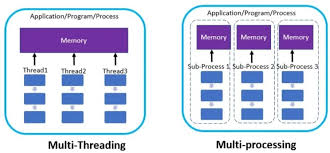
\includegraphics[width=0.7\textwidth]{mp vs mt.jpg}
    \end{center}

    Multiple threads can run inside one parent process. Operating system schedules processes and threads across available cores
    \newpage
    \begin{itemize}
        \item Why prefer multi-processing over multi-threading? Data races. A Julia example:
        \begin{jllisting}
using Base.Threads

winner = 0
@threads for i in 1:10
    winner = i
end
@show winner
        \end{jllisting}
        \item \texttt{winner} is indeterminate. What would happen in mutli-processing?
    \end{itemize}
    \newpage

    \begin{itemize}
        \item A third model to understand is \textit{cooperative multitasking}
        \pause
        \item When making API calls, your computer is just waiting while the server responds
        \item Why not fire off more requests while waiting for the response?
        \pause
        \item Single \textit{thread}, multiple \textit{tasks}
        \pause
        \item For IO-bound applications (whereas multi-threading/processing is for CPU-bound)
        \item See \texttt{asyncio} and \texttt{aiohttp} in Python for the curious
    \end{itemize}
\end{frame}

\begin{frame}[allowframebreaks,fragile]{Loops vs. Implicit Parallelization}
    \begin{itemize}
        \item Implicit parallelization: when programming language allows compiler or interpreter to automatically exploit parallelism inherent to a problem through the language's constructs.
        \begin{lstlisting}[language=Python]
import numpy as np

x = np.random.normal(0,1,10**7)  # 10 million random draws
y = np.square(x)                 # takes 0.05 seconds on my PC
y = x**2                         # about the same;
                                 # numpy overrides standard math operators,
                                 # invokes implicitly parallelized functions
y = np.zeros(x.shape[0])
for i in range(x.shape[0]):
    y[i] = x[i]**2               # takes 2.96 seconds on my PC
        \end{lstlisting}
        \item Avoid loops wherever possible.  Leverage implicit parallelization with vectorization and broadcasting.
        \newpage
        \item ``Vectorization'' in high-level language (e.g. python, matlab, julia) means use of optimized, pre-compiled code in low-level language (e.g. C) to perform mathematical operations over sequence of data.
        \item E.g. numpy takes advantage of homogenous dtype in an array to delegate task of performing mathematical operations on array's contents to pre-compiled C code.
        \item Examples: square (unary); np.maximum (binary); np.sum (sequential)
        \begin{lstlisting}[language=Python]
import numpy as np

x = np.random.normal(0,1,10**7)  # 10 million random draws
y = np.sum(x)                    # takes 0.02 seconds on my PC

y = 0
for i in range(x.shape[0]):
    y += x[i]                    # takes 1.91 seconds on my PC
        \end{lstlisting}
        \item Most numpy math functions are ``vectorized,'' including logical and LA functions.
    \end{itemize}
\end{frame}

\begin{frame}[allowframebreaks,fragile]{Broadcasting}
    \begin{itemize}
        \item Mechanism allowing arrays of unequal shapes to be used in vectorized operations.
        \item Effectively ``stretches'' arrays to replicate contents along chosen dimensions, such that higher-dim array suits the operation.
        \item Enables element-wise calculation across otherwise incompatible shapes.
        \item E.g. let's raise a length-10 vector to powers (element-wise) contained in the columns of a (10, 10 million) matrix.
        \end{itemize}
        
        \newpage
        
        \begin{lstlisting}[language=Python]
import numpy as np

X = np.random.uniform(1,2,size=(10,10**7))
Y = np.random.uniform(2,10,size=10)

Z = Y**X                          # ValueError: operands could not be broadcast  
                                  # together with shapes (10,) (10,10000000)
Z = np.zeros((X.shape))
for i in range(X.shape[1]):
    Z[:,i] = Y**X[:,i]            # could do it this way, takes 43.5 seconds

Z = Y[:,None]**X                  # broadcasting is MUCH faster: 8.9 seconds
        \end{lstlisting}
    \begin{itemize}
        \item Gains are magnified over larger loops and more complicated calculations.
        \item Might have many such instances in a single structural model.  Utilizing implicit parallelization in place of loops can make tractable an otherwise intractable model.
    \end{itemize}
\end{frame}

\section{Languages}

\begin{frame}[fragile]{Julia}
    \begin{jllisting}
using Distributed; addprocs(4)

@everywhere begin
    using Statistics
    a = 4
end

pmap(1:100) do i
    mean(randn(a)) * i
end
    \end{jllisting}
\end{frame}

\begin{frame}[fragile]{R}
    \begin{lstlisting}[language=R]
library(parallel)

cl <- makePSOCKCluster(4)
a <- 4

clusterExport(cl, "a")

parSapply(cl, 1:100, function(i) mean(rnorm(a)) * i)
    \end{lstlisting}
\end{frame}

\begin{frame}[fragile]{Python}
    \begin{lstlisting}[language=Python]
import numpy as np, functools
from multiprocessing import Pool

def par_func(rng,a,i):
    return np.mean(rng.normal(size=a))*i

def outer(n_procs):
    rng = np.random.default_rng(1)
    a = 4
    with Pool(n_procs) as p:
        p.map(functools.partial(par_func,rng,a),np.arange(1,100).tolist())

if __name__ == '__main__':
    outer(4)
    \end{lstlisting}
    \begin{itemize}
        \item Avoid referring to globally defined objects, pass all function inputs explicitly to child processes (as in Julia and R) by freezing into function signature.
        \item This is ``best practice'' for pseudo-random number generation in \verb|numpy|, but \emph{not} when the PRNGs are being drawn in parallel.  More on this later. 
    \end{itemize}
\end{frame}

\begin{frame}[fragile]{Matlab}
    \begin{lstlisting}
clear; clc; 

a = 4;
P = 4;
pool = parpool('local', P);

parfor i = 1:100
    mean(randn(a,1)) * i
end

delete(pool);
    \end{lstlisting}
\end{frame}

\section{Example in Python: Multinomial Choice}
\begin{frame}{Example: Multinomial Choice Problem - Setup}
    \begin{itemize}
        \item 100,000 consumers $i$, each with an observed scalar individual characteristic $W_i$.
        \item 10 product choices $j$, each with scalar product characteristic $X_j$.
        \item Unobserved consumer-specific component of indirect utility $S_i$ is i.i.d. std. normal
        \item Use 1,000 simulation draws $S_{is}$ for each consumer to form a simulated likelihood.
        \item Assuming parameters $\beta = (\beta_0,\beta_1,\beta_2,\beta_3)$, indirect utility for $i$-th consumer, $j$-th product and $s$-th simulant is
        \[
        U_{ijs} = \beta_0 + (\beta_1 + \beta_2 W_i + \beta_3 S_{is})X_j + \epsilon_{ijs}
        \]
        \item $\epsilon_{ijs}$ is idiosyncratic unobserved utility, assumed distributed type-1 extreme value.
        \item Draw $(X_j,W_i,S_{is})$, generate fake consumer choices and parameters.
        \item Parallelize formation of likelihood over consumer-choice pairs, integrating-out simulants to compute CCPs.
    \end{itemize}
\end{frame}

\begin{frame}[fragile]{Multinomial Choice (python + multiprocessing): DGP}
    \begin{lstlisting}[language=Python]
import numpy as np
from multiprocessing import Pool
import functools

def data():
    N_cons = 100000                            # 100,000 consumers (W)
    N_choices = 10                             # 10 choices (X)
    N_sims = 1000                              # 1000 sim draws (S)
    W = np.random.uniform(0,1,N_cons)
    X = np.random.uniform(0,1,N_choices)[:,None]
    S = np.random.normal(0,1,N_sims)[None,:]   # prep for broadcasting
    Y = np.random.randint(0,10,N_cons) + 1     # 100k consumer choices (Y) 
    prod_IDs = np.arange(10).astype(int) + 1   # product IDs 1-10
                                               # match choices to prod. IDs
                                               # to create binary choice matrix
    aux = Y[:,None] / prod_IDs[None,:]         # (N_cons x N_prods)
    choices = np.zeros((aux.shape[0],aux.shape[1]))
    choices[aux==1] = 1
    beta = np.random.uniform(0,1,4)            # fake parameters
    W_list = W.tolist()                        # send W to list for p.map
    return W_list, X, S, choices, beta
    \end{lstlisting}
\end{frame}

\begin{frame}[fragile]{Multinomial Choice (python + multiprocessing): Compute Likelihood}
    \begin{lstlisting}[language=Python]
def comp_CCP(X,S,beta,W_list):
    e_util_ijs = np.exp(beta[0] + (beta[1] + beta[2]*W_list + beta[3]*S)*X)
    CCP_ijs = e_util_ijs/np.sum(e_util_ijs,axis=0) # compute CCPs after broadcast
    CCP_ij = np.mean(CCP_ijs,axis=1)               # integrate-out simulants
    return CCP_ij                                  # length-10 vector for i

def total_LL(n_processes):
    W_list, X, S, choices, beta = data()
                            # freeze inputs into CCP function signature
    partial_comp_CCP = functools.partial(comp_CCP,X,S,beta)
    with Pool(n_processes) as p:        # call process pool
                            # p.map takes iterable of consumer characteristics
                            # and generates list of CCP function outputs
        CCP_ij = np.vstack(p.map(partial_comp_CCP,W_list))
        total_LL = np.sum(choices*np.log(CCP_ij) + (1-choices)*np.log(1-CCP_ij))
    return total_LL
                                # need to declare main module, any calls above
if __name__ == '__main__':      # are sent to child processes and duplicated
    n_processes = 20            # allocate 20 cores (of 40 available on VM)
    tot_LL = total_LL(n_processes)
    \end{lstlisting}
\end{frame}

\begin{frame}[allowframebreaks,fragile]{Multinomial Choice (python): Discussion}
    \begin{itemize}
        \item Runs in 1.1 seconds on 20 cores.
        \item ``Serial'' implementation (also iterating over consumers, but ``mapped'') takes about 11 seconds.
        \item Or, vectorize/broadcast to avoid the loop over consumers? Work in 3D: 
        \begin{lstlisting}[language=Python]
W = np.random.uniform(0,1,N_cons)[:,None,None]
X = np.random.uniform(0,1,N_choices)[None,:,None]
S = np.random.normal(0,1,N_sims)[None,None,:]
    # other corresponding modifications to functions...
    # (see Github repository for code)
        \end{lstlisting}
        \item Takes about 30 seconds.  Why?  We said broadcasting was faster than a loop.
        \item The issue is \verb|np.exp| of 3D tensor.  Only 10s of operation is broadcast to produce 3D tensor, other 20s is exponential of it.

        \newpage
        \item Some \verb|numpy| functions (powers especially) don't vectorize well into high-dimensions. Lots of overhead.
        \item Numerical example:
        \begin{verbatim}
np.exp time over 100 runs, 10^6 draws: 10.19 ms
mapped math.exp time over 100 runs, 10^6 draws: 0.00026 ms     
for-loop math.exp time over 100 runs, 10^6 draws: 339.47 ms
        \end{verbatim}
        \item  \verb|map| is 39,000 times faster than \verb|np.exp|; 1.3 million times faster than true serial implementation.
        \begin{itemize}
            \item \verb|map| "works as an iterator to return a result after applying a function to every item of an iterable."
            \item Still iterating, but effectively manually vectorizes function onto iterable.
        \end{itemize}
        \item \verb|np.exp| is implicitly parallel but still slower.
        \item A true serial (for-loop) implementation over consumer features in MNC problem would take too long, haven't computed it.

        \newpage
        \item Broadcasting works well in high-dimensions with matrix algebra:
        \begin{itemize}
            \item \verb|matmul|, 
            \item broadcast operations over arrays, etc.
            \item Depending on operation, should try different approaches.
        \end{itemize}
        \item Taking exponents of a 3D matrix is inherent challenge to computing CCPs (per guess of params) in estimating RC logit demand models with product features and both observed and unobserved individual heterogeneity. 

        \newpage
        \item Workarounds include:
        \item Iterating over a dimension and taking exponentials of 2D matrices.  This should be further optimized:
        \begin{itemize}
            \item Use \verb|map| to ``manually vectorize'' (as above)
            \item \verb|flatten| a dimension + \verb|bincount| $\rightarrow$ 2D, no loop
        \end{itemize}
        \item And/or ``just-in-time'' compilation: native machine level code optimized to your functions (compile to GPU or CPU); what Julia + Matlab do automatically.  Powerful.
        \item In Python: \verb|jax| and \verb|numba| packages.
        \item \verb|jax.jit| compiling the CCP and likelihood calc. over 3D takes 3.8 seconds (vs. 30).
        \item Good idea to use \verb|jit|-compilation in large problems. Need to try \verb|jit| with \verb|map| to further optimize MNC example.

        \newpage
        \item In many situations, you would not be able to replace your entire parallelized operation with broadcasting anyway; need a loop.
        \item Gains from parallelization can be even larger in real-world problems, depending on what you're parallelizing.
        \item E.g. bootstrap; iterating over estimation starting points; simulations; running regressions on many separate datasets.
        \item Key is the operation needs to be ``parallelizable:'' Passing \emph{many} objects separately through one process (process can change given the iterable).
        \item Process pool can handle multiple iterables: \verb|Pool.starmap| in python, or package into a list of tuples and use \verb|Pool.map|. Read more, here (\href{https://docs.python.org/3/library/multiprocessing.html#multiprocessing.pool.Pool}{link}).
    \end{itemize}
\end{frame}

\section{Extras}

\begin{frame}{Resource Monitoring}
    \begin{itemize}
        \item Windows: Ctrl+Alt+Del (Task Manager); Mac: Activity Monitor
        \item Mac, Linux and Cygwin Terminals: \texttt{top}/\texttt{htop}
        \begin{center}
            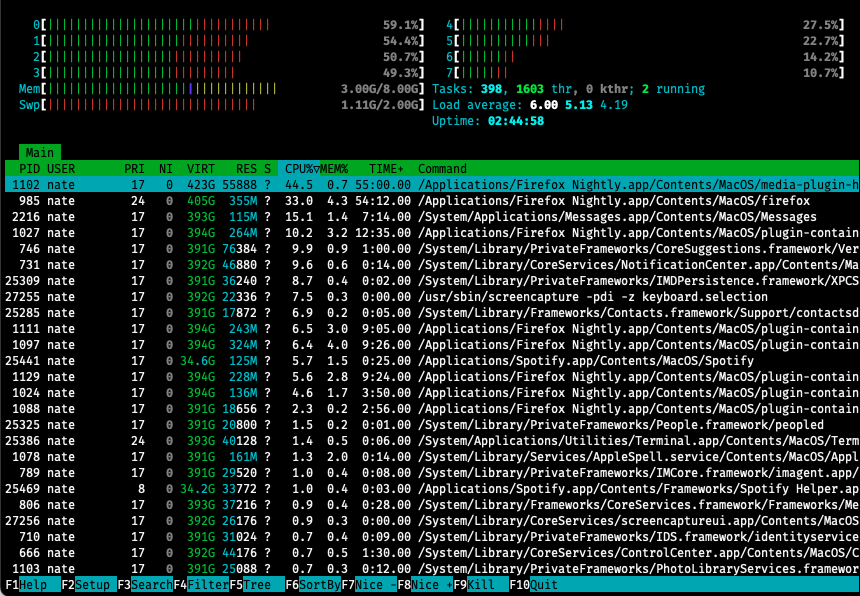
\includegraphics[width=0.5\textwidth]{htop.png}
        \end{center}
        \item Control output of top with your keyboard (\href{https://opensource.com/article/18/8/top-tips-speed-up-computer}{link})
    \end{itemize}
\end{frame}

\begin{frame}[fragile]{File Transfer to VM}
    \begin{itemize}
        \item Option 1: Use \verb|scp| from command line.  Refer to account on VM as <EID>@ovrw-econ-p02.la.utexas.edu.
        \item Note: This is the address for the IO VM. Other research fields have separate VM allocations; the address will differ slightly.
        \item Option 2: Use a GUI \verb|scp| client like WinSCP.
        \item Option 3: \verb|RDP| local mirror. Access local files in a remote session through your PC's remote desktop GUI.  Instructions differ slightly for Windows (\href{https://www.thesagenext.com/support/access-local-drive-files-from-remote-desktop-session}{link}) and Mac (\href{https://ticket.summithosting.com/hc/en-us/articles/360041678333-RDP-Adding-Local-Drives-Devices-Mac-OS-X}{link}).
        \item DO NOT use Box Drive or the Box website.  You may be prompted to log into Box Drive upon accessing the VM.  Ignore the prompt.
    \end{itemize}
\end{frame}


\begin{frame}{Memory Management}
    \begin{itemize}
        \item Point 1: What is RAM? What is disk memory?
        \pause
        \item Point 2: Size on disk $\ne$ size in RAM
        \pause
        \item Point 3: Multiple processes $\implies$ duplicate memory
        \pause
        \item Conclusion: Be careful! Know your RAM limits!
        \pause
        \item Example: ML packages that bootstrap
    \end{itemize}
\end{frame}

\begin{frame}[fragile,allowframebreaks]{Memory Tips}
    \begin{itemize}
        \item Julia and R: Only pass chunks of your dataframe (if $\sim$two copies fit in memory)
        \begin{jllisting}
using CSV, DataFrames, Distributed

df = CSV.read("really-big-file.csv") |> DataFrame

pmap(eachrow(df)) do row
    # do things with row...
end
        \end{jllisting}
        \item Python can do similar: use \verb|pandas.iterrows|. Still not copying df to child processes.
        \newpage
        \item An alternative: \textit{don't} load the file, pass indices to subprocesses and have subprocesses load parts of the file using limit/offset arguments
\begin{lstlisting}[language=Python]
from multiprocessing import Pool
from math import ceil
import pandas as pd
from functools import partial

def process_batch(N, B, batch_num):
    offset = batch_num * B
    limit = B if offset + B < N else N - offset
    df = pd.read_csv("really-big-file.csv", skiprows = offset, nrows = limit)
    # do something with df...

if __name__ == '__main__':
    BATCH_SIZE = 1000
    N_ROWS = # however many rows your CSV has
    f = partial(process_batch, N_ROWS, BATCH_SIZE)
    with Pool(4) as p:
        p.map(f, range(ceil(N_ROWS / BATCH_SIZE)))
\end{lstlisting}
\newpage

\item Chunked (aka batched) reading is another way to process very large files
\begin{itemize}
    \item \texttt{chunksize} in the \texttt{pandas.read\_csv} function (\href{https://stackoverflow.com/questions/25962114/how-do-i-read-a-large-csv-file-with-pandas}{link})
    \item \text{read\_csv\_chunked} in R (\href{https://readr.tidyverse.org/reference/read_delim_chunked.html}{link})
    \item \text{CSV.Chunks} in Julia (\href{https://csv.juliadata.org/stable/reading.html#CSV.Chunks}{link})
    \item \texttt{datastore} in Matlab (\href{https://www.mathworks.com/help/matlab/ref/datastore.html}{link})
\end{itemize}
\item This is about memory management, \textit{not} parallel processing{\textemdash}these functions read one portion of the file at a time. Need to figure out how to add parallelization on top if this is important for performance
\item The Python example code on previous slide is effectively parallel batch processing\dots
    \end{itemize}
\end{frame}

\begin{frame}{Cluster Access}
    \begin{itemize}
        \item We also have access to one of the world's largest supercomputers at TACC
        \item Need a prof to sponsor you as PI and pay for an allocation
        \item This is a \textit{cluster} of computers
        \item Controlled by Simple Linux Utility for Resource Management (SLURM)
        \item For when your computational problems get really big
    \end{itemize}
\end{frame}

\begin{frame}[fragile,allowframebreaks]{Pseudo-Random Number Generation}
    \begin{itemize}
        \item ``Random'' numbers generated by a computer only approximate a stochastic process. Sequence generated deterministically from an initial seed.
        \item How do we seed an RNG so it is reproducible?  And how do we do it in parallel?
        \item In the initial Python multiprocessing example, we seeded a single RNG that can be passed to functions: best-practice (vs. global RNG) outside of parallel environments.
        \item But in parallel, the RNG is passed to each child process so the draws are the same on each child process.
        \item Unlikely this is what you want; would be more efficient to draw the random numbers before the parallel process and pass those draws to the child processes.
        \item Answer is to spawn a \verb|SeedSequence| and child seeds (equal to number of child processes) from it and RNGs from those, then pass those RNGs to the child processes.
        \item More on the hazards and best practices of PRNG in parallel (\href{https://blog.scientific-python.org/numpy/numpy-rng/}{link 1}, \href{https://numpy.org/doc/stable/reference/random/parallel.html}{link 2}).
        \newpage
        \item In Julia, the ability to control how you send variables to subprocesses lets you control whether or not the draws are the same in subprocesses.\\
        \begin{jllisting}
using Distributed; addprocs(2)
            
@everywhere seed = randn()
@info "Same" seed_one=@fetchfrom(2, seed) seed_two=@fetchfrom(3, seed)

@info "Different" seeds = pmap(1:5) do i
    i => (procid = myid(), x = randn())
end
        \end{jllisting}
    \end{itemize}
\end{frame}

\begin{frame}{Github Repository}
    \begin{itemize}
        \item Github repository (\href{https://github.com/nateybear/parallel-racers}{link}) with all of our code.
        \item Includes Python, Matlab, Julia and C implementations of the MNC problem.
        \item Also speed comparisons across languages and methods on a binomial choice, Rust (1987)-inspired likelihood calculation.
        \item Corresponding Wiki (\href{https://github.com/nateybear/parallel-racers/wiki}{link}), includes some details which expand on these slides.
    \end{itemize}
\end{frame}


\end{document}